%Dies ist die Hauptseite des Dokumentes. Es werden u. a. alle Kapitel,
%Einstellung im Header eingebunden.  Veränderungen müssen in folgenden Dateien
%vorgenommen werden:
      %- config.tex
      %- einzelne Kapitel (evtl. erweitern)

%Hier sind alle Einstellungen enthalten, die sich auf das Seiten- und
%Dokumentenlayout beziehen

\documentclass[
  11pt,                   % Schriftgröße
  DIV12,
  german,                 % für Umlaute, Silbentrennung etc.
  oneside,                % einseitiges Dokument
  titlepage,              % es wird eine Titelseite verwendet
  parskip=half,           % Abstand zwischen Absätzen (halbe Zeile)
  headings=normal,        % Größe der Überschriften verkleinern
  captions=tableheading,  % Beschriftung von Tabellen unterhalb ausgeben
  final                   % Status des Dokuments (final/draft)
]{scrreprt}               %


%------Ändern von Schriftschnitten - (Muss ganz am Anfang stehen !) ------------
\usepackage{fix-cm}


%------Umlaute -----------------------------------------------------------------
%   Umlaute/Sonderzeichen wie äüöß können direkt im Quelltext verwenden werden.
%    Erlaubt automatische Trennung von Worten mit Umlauten.
\usepackage[T1]{fontenc}
\usepackage[utf8]{inputenc}

%------Anpassung der Landessprache----------------------------------------------
\usepackage[ngerman]{babel}

%------Einfache Definition der Zeilenabstände und Seitenränder------------------
\usepackage{geometry}
\usepackage{setspace}

%------Schriftgrößenanpassung von einzelnen Textpassagen------------------------
\usepackage{relsize}

%------Trennlinien in Kopf- und Fusszeile
\usepackage[headsepline, footsepline, ilines]{scrlayer-scrpage}

%------Grafiken und Farben -----------------------------------------------------
\usepackage{graphicx}

%------Packet zum Sperren, Unterstreichen und Hervorheben von Texten------------
\usepackage{soul}

%------ergänzende Schriftart----------------------------------------------------
\usepackage{helvet}

%------Lange Tabellen-----------------------------------------------------------
\usepackage{longtable}
\usepackage{array}
\usepackage{ragged2e}
\usepackage{lscape}
\usepackage{tabularx}

%------DocTeX-------------------------------------------------------------------
\usepackage{changepage}
\usepackage{scalerel}
\newcolumntype{R}{>{\raggedright\arraybackslash}X}%

%------PDF-Optionen-------------------------------------------------------------
\usepackage[
  bookmarks,
  bookmarksopen=true,
  colorlinks=true,
  linkcolor=black,        % einfache interne Verknüpfungen
  anchorcolor=black,      % Ankertext
  citecolor=black,        % Verweise auf Literaturverzeichniseinträge im Text
  filecolor=black,        % Verknüpfungen, die lokale Dateien öffnen
  menucolor=black,        % Acrobat-Menüpunkte
  urlcolor=black,         % Farbe für URL-Links
  backref,                % Zurücktext nach jedem Bibliografie-Eintrag als
                          % Liste von Überschriftsnummern
  pagebackref,            % Zurücktext nach jedem Bibliografie-Eintrag als
                          % Liste von Seitenzahlen
  plainpages=false,       % zur korrekten Erstellung der Bookmarks
  pdfpagelabels,          % zur korrekten Erstellung der Bookmarks
  hypertexnames=false,
  colorlinks=true,   % zur korrekten Erstellung der Bookmarks
  linktocpage             % Seitenzahlen anstatt Text im Inhaltsverzeichnis verlinken
  ]{hyperref}
  \hypersetup{
    colorlinks=true, %set true if you want colored links
    linktoc=all,     %set to all if you want both sections and subsections linked
  }
  \usepackage{verbatim}
  \usepackage{lipsum}                     % Dummytext
  \usepackage{xargs}                      % Use more than one optional parameter in a new commands
  \usepackage[pdftex,dvipsnames]{xcolor}  % Coloured text etc.

  \usepackage[colorinlistoftodos,prependcaption,textsize=tiny]{todonotes}

%------Glossar------------------------------------------------------------------
\usepackage[translate=babel,toc]{glossaries}
      % enthält eingebundene Packete

%------Seitenränder-------------------------------------------------------------
\geometry{verbose,                     % zeigt die eingestellten Parameter beim
                                       % Latexlauf an
      paper=a4paper,                   % Papierformat
      top=25mm,                        % Rand oben
      left=25mm,                       % Rand links
      right=25mm,                      % Rand rechts
      bottom=45mm,                     % Rand unten
      pdftex                           % schreibt das Papierformat in die
                                       % Ausgabe damit Ausgabeprogramm
                                       % Papiergröße erkennt
  }

%Seitenlayout
\onehalfspace        % 1,5-facher Abstand

%------Kopf- und Fußzeilen -----------------------------------------------------
\pagestyle{scrheadings}

%------Kopf- und Fußzeile auch auf Kapitelanfangsseiten ------------------------
\renewcommand*{\chapterpagestyle}{scrheadings}

%------Schriftform der Kopfzeile -----------------------------------------------
\renewcommand{\headfont}{\normalfont}

%----Spezielle Befehle
\newcommand{\lfk}[1]{$\langle LF#1\rangle$}

%----Farben
\definecolor{tubsRed}{cmyk}{0.1,1.0,0.8,0.0}
\definecolor{tuRed}{cmyk}{1.0,0.0,0.6,0.0}

%------Kopfzeile----------------------------------------------------------------
\setheadsepline{1pt}[\color{tuRed}]
\setlength{\headheight}{21mm}        % Höhe der Kopfzeile
\ihead{\large{\textsc{\praktikumTitel}}\\    % Text in der linken Box
       \small{\projektTitel}}
\chead{}                            % Text in der mittleren Box

%----Fusszeile
\setfootsepline{1pt}[\color{tuRed}]
\cfoot{}                            % Text in mittlerer Box
\ofoot{\pagemark}                    % Seitenzahl in rechter Box



%------Labels mit eigenem Text für \ref ----------------------------------------
\makeatletter
\def\namedlabel#1#2{\begingroup
#2%
\def\@currentlabel{#2}%
\phantomsection\label{#1}\endgroup
}
\makeatother


%------Neue Environments -------------------------------------------------------

\newcommand{\refsetcounter}[2]{\setcounter{#1}{#2}\addtocounter{#1}{-1}\refstepcounter{#1}}

%Funktion im Pflichtenheft
\newcounter{functioncount} 
\newenvironment{function}[2]{\refsetcounter{functioncount}{#1}\large\textbf{\sffamily{#2 }}\namedlabel{F#1}{$\langle F#1\rangle$}\normalsize\begin{description}\setlength{\itemsep}{-5pt}}{\end{description}}

%Daten im Pflichtenheft
\newcounter{datacount}
\newenvironment{data}[2]{\refsetcounter{datacount}{#1}\textbf{#2} \namedlabel{D#1}{$\langle D#1\rangle$}\\}{}

%Kriterien im Pflichtenheft
\newcounter{mustcount} 
\newcommand{\must}[2]{\refsetcounter{mustcount}{#1}\namedlabel{RM#1}{$\langle RM#1\rangle$} #2\\}

\newcounter{wishcount}
\newcommand{\wish}[2]{\refsetcounter{wishcount}{#1}\namedlabel{RW#1}{$\langle RW#1\rangle$} #2\\}

\newcounter{notfunctional}
\newcommand{\notfunctional}[2]{\refsetcounter{notfunctional}{#1}\namedlabel{NF#1}{$\langle NF#1\rangle$} #2\\}

\newcommand{\wont}[2]{\refsetcounter{datacount}{#1}\namedlabel{RN#1}{$\langle RN#1\rangle$} #2\\}

%Qualitätsanforderungen im Pflichtenheft
\newcommand{\qualityReq}[2]{\refsetcounter{datacount}{#1}\namedlabel{Q#1}{$\langle Q#1\rangle$} #2\\}

% Benutzeroberflächen im Pflichtenheft
\newcounter{uicount}
\newenvironment{ui}[2]{\refsetcounter{uicount}{#1}\textbf{#2} \namedlabel{UI#1}{$\langle UI#1\rangle$}\\}{}

% Klassen
\newcounter{classcount}
\newenvironment{class}[2]{\refsetcounter{classcount}{#1}\textbf{#2}\namedlabel{CL#1}{$\langle CL#1\rangle$}\begin{description}\setlength{\itemsep}{-5pt}}{\end{description}}

% Entitäten
\newcounter{entitycount}
\newenvironment{entity}[2]{\refsetcounter{entitycount}{#1}\textbf{#2} \namedlabel{E#1}{$\langle E#1\rangle$}\\}{}

% Component
\newcounter{componentcount}
\newenvironment{component}[2]{\refsetcounter{componentcount}{#1}\textbf{Komponente \namedlabel{C#1}{$\langle C#1\rangle$}: #2}\\}{}

% Interface
\newcounter{interfacecount}
\newenvironment{interface}[2]{\refsetcounter{interfacecount}{#1}\textbf{Schnittstelle \namedlabel{I#1}{$\langle I#1\rangle$}: #2}\\}{}

% Testfall
\newcounter{testcasecount}
\newenvironment{testcase}[2]{\refsetcounter{testcasecount}{#1}\textbf{Testfall #2}\namedlabel{T#1}{$\langle T#1\rangle$}\normalsize\begin{description}\setlength{\itemsep}{-5pt}}{\end{description}\hspace{7.5em}}
           % Diese Datei enthält alle
                                           % Layouteinstellungen
\newcommand{\dokumentTitel}{Pflichtenheft}
% Definition von globalen Parametern, die derzeit auf der Titelseite und in der
% Kopfzeile verwendet werden. Der in <> gesetzte Text ist zu verändern.

\newcommand{\praktikumTitel}{Praxis der Softwareentwicklung}
\newcommand{\projektTitel}{Solidarische Raumnutzung}

\newcommand{\semester}{Wintersemester 2024/25}
\newcommand{\institut}{
	Institut für Anthropomatik und Robotik (IAR)\\
	Forschungsgruppe Mensch-Maschine-Interaktion und Barrierefreiheit (MBI)\\
	Prof. Dr. Kathrin Gerling\\
	Adenauerring 10, Gebäude 50.28\\
	76131 Karlsruhe\\
}
\newcommand{\institutsLogo}{common/hci.png}
\newcommand{\kitlogo}{common/kit_logo.jpg}
\newcommand{\betreuer}{Sabrina Burtscher}


\makeglossaries

%------Beginn des Gesamtdokumentes----------------------------------------------
\begin{document}

%------Eingebundene Seiten, Verzeichnisse bzw. Kapitel--------------------------
% Dies ist die Titelseite.
% Die Ausgabe darf 1 Seite nicht überschreiten, also ggf. Abstände anpassen
% Die Angabe in [...] gibt den Abstand nach der entsprechenden Zeile an.


%----Stil dieser Seite----------------------------------------------------------
\thispagestyle{plain}      % Kopfzeile bleibt leer

%----Beginn der Titelseite------------------------------------------------------
\begin{titlepage}

\vspace*{-3.8cm}
\hspace*{-2cm}\begin{minipage}{1.25\textwidth}

\includegraphics[width=5.3cm]{common/kit_logo}\setlength{\unitlength}{1mm}\begin{picture}(00,00)(-10,0)\color{tuRed}\put(000,004){\line(1,0){140}}\end{picture}%\hfill
\parbox[b]{0.68\textwidth}{\hfill\includegraphics[width=8cm,height=2.4cm,keepaspectratio]{\institutsLogo}\\~}
\end{minipage}


~\\[5ex]

%----zentrierte Ausrichtung über die gesamte Seite----------------------------
\begin{center}

%----Titel des Praktikum (\praktikumTitel in newComments zu verändern)--------
{\relsize{4}{\textbf{\textsc{\praktikumTitel}}}}\\[5ex]

%----Titel des Teilprojektes (\projektTitel in newComments verändern)---------
{\relsize{3}{\textbf{\textsc{\projektTitel}}}}\\[5ex]

Praxis der Softwareentwicklung (PSE)\\
\semester\\[6ex]

{\relsize{3}{\textbf{\dokumentTitel}}}\\[5ex]

%----Daten des Auftraggebers
Karlsruher Institut für Technologie (KIT)\\
\institut[2ex]
\textbf{Betreuer: \betreuer}\\[5ex]

\textbf{Projektteilnehmer:}\\

% ----Tabelle der Praktikumsteilnehmer------------------------------------------
\begin{tabular}{l<{\hspace{20mm}} l<{\hspace{30mm}}}\\
  Name                   &   E-Mail-Adresse\\      % Zeilenüberschift

  \hline                    % Linie unterhalb der Zeilenüberschrift

  %----Nachfolgend alle Namen und E-Mail-Adressen der Teilnehmer einfügen
  Antonia Ammon  &  <E-Mail-Adresse>\\
  Ben Steinle &  <E-Mail-Adresse>\\
  Johannes Frohnmeyer &  <E-Mail-Adresse>\\
  Alexander Klee &  <E-Mail-Adresse>\\
  Jannik Hönlinger &  <E-Mail-Adresse>\\

\end{tabular}

%Zur Vereinheitlichung sollten hier die TU Braunschweig Emailadressen benutzt werden. % enthält Tabelle der Praktikumsteilnehmer

\vfill
Karlsruhe, \today

\end{center}
\end{titlepage}
                       % Titelseite

%!TEX root = ../Pflichtenheft.tex

\chapter{Glossar}

\begin{description}
\item[CI/CD] Baut automatisiert Software, führt Tests durch und veröffentlicht Artefakte
\item[Docker] Software zur Bereitstellung von Anwendungen innerhalb von Containern
\item[Container] Isolierte Umgebung um Software unabhängig von der zugrunde liegenden Umgebung auszuführen
\item[Browser] Software zum Navigieren von Webseiten, zum Beispiel Firefox oder Chrome
\item[Git] Software zur Versionsverwaltung von Softwareprojekten
\item[GitHub] Plattform zur Versionsverwaltung von Softwareprojekten, nutzt Git
\item[IDE] (Integrated Development Environment) Software, welche alle Werkzeuge zur Softwareentwicklung in einem Programm kombiniert
\item[AMD64] Verbreitete Prozessorarchitektur von Intel und AMD
\item[RAM] (Random Access Memory) Arbeitsspeicher
\item[VM] (Virtuelle Maschine) Software zur Simulation eines Computers
\item[PostgreSQL] Objekt-Relationales Datenbankmanagementsystem, welches zum Speichern und Verwalten von Daten verwendet wird
\item[HTML] (Hypertext Markup Language) Eine Sprache um die Struktur und den Inhalt einer Website zu definieren
\item[CSS] Cascading Style Sheets, ist eine Sprache um das Visuelle aussehen einer Website zu definieren
\item[JavaScript] Programmiersprache um das Logische verhalten von Webseiten zu steuern
\item[SSR] (Server-Side Rendering) Methode um das HTML einer Website auf dem Server zu produzieren, anstelle des Browsers
\item[REST] (Representational State Transfer) Architekturstil von APIs für das Internet
\item[API] Schnittstelle auf Quelltext-Ebene um anderen Programmen funktionen zur Verfügung zu stellen
\item[OIDC] (OpenID Connect) Authorisierungsframework welches vom KIT genutzt wird um dritten Webseiten Logins basierend auf KIT-Konten bereitzustellen
\end{description}

\tableofcontents                           % Inhaltsverzeichnis wird automatisch
                                           % generiert
\listoffigures
\newpage
%\listoftodos[Notes]
%----Kapitel des Pflichtenhefts, die mit Inhalt zu füllen sind--------------------
%!TEX root = ../Pflichtenheft.tex
\chapter{Einleitung}
In modernen und inklusiven Arbeits- und Lernumgebungen spielen Rückzugsorte eine zentrale Rolle um produktives Arbeiten und das Wohlbefinden aller gewährleisten zu können.
Das Institut für Mensch-Maschine-Interaktion und Barrierefreiheit (MIB) am KIT bietet einen Ruheraum, welcher für Meetings, kurzen Pausen oder als Rückzugsort nach einer Reizüberflutung genutzt werden kann.

Derzeit wird der Status des Raumes durch ein einfaches Türschild angezeigt, welches lediglich den Status \textit{verfügbar} oder \textit{besetzt} anzeigt.
Dieses System bietet jedoch keine Möglichkeit, die Dringlichkeit sowie die Nutzung zu kommunizieren und zu planen.

Im Rahmen dieses Projekts wird ein innovatives Buchungssystem entwickelt, das über ein klassisches \textit{frei}- oder \textit{gebucht}-System hinausgeht.
Ziel ist es, ein System zu schaffen, das es den Nutzer*innen ermöglicht, ihre Bedürfnisse differenziert anzugeben.
Dadurch soll eine transparente und flexible Abstimmung über die Raumnutzung ermöglicht werden, die sowohl individuellen Bedürfnissen als auch einer optimalen Raumverteilung gerecht wird.
%!TEX root = ../Pflichtenheft.tex
\section{Allgemeine Hinweise}
\textbf{Template} Tragen Sie vor Beginn der Ausarbeitung Ihre Daten in die Datei 'common/teilnehmer.tex' ein. Löschen Sie die Template-Texte und -Bilder, sobald Sie Ihren Text geschrieben haben.

\textbf{Anglizismen} Verwenden Sie ruhig die englischen Wörter.

\textbf{Fett-/Kursivschreibweise} Entscheiden Sie sich zu Beginn innerhalb der Gruppe, wann Sie \textit{kursive} und wann Sie \textbf{fette} Schrift einsetzen möchten.

\textbf{Bilder} Legen Sie eigene Bilder stets im 'figures' Ordner ab. Nutzen Sie die im Template beispielhaft eingebundenen Bilder als Vorlage. Außerdem erlaubt Overleaf das Einfügen von Bildern im GUI (siehe obere Task-Leiste).


\chapter{Zielbestimmung}
\label{chap:target}
\improvement[inline]{Dieser Abschnitt sollte noch ausführlicher beschrieben werden.}
Dieser Abschnitt hat die Aufgabe, als eine Art Einleitung zu dienen. Es soll
ein kurzer Umriss über Ziel und Motivation des Gesamt- und ggf. der
Teilprojekte dargestellt werden. Beschrieben wird die Hauptaufgabe des Systems.
Wichtig ist, den Grund für die Systementwicklung (Probleme oder Geschäftsidee)
und damit ihre Ziele herauszuarbeiten.

\todo[inline]{The original todo note withouth chaflsjklfsdkljnged colours.\newline Here's another line.}
\section{Musskriterien}\label{sec:musskriterien}
In diesem Abschnitt halten wir unabdingbare Leistungen der Software fest\\
Wir halten also welche Funktionalitäten/Leistungen das Softwareprodukt in
jedem Fall erfüllen muss, damit es genutzt werden kann.
\todo[inline]{Hier fallen uns noch sicherliche mehr Kriterien ein.}
\must{1}{Die Anwendung soll als Web-Applikation realisiert werden.}
\must{2}{Die Anwendung soll schnell und einfach bedienbar sein.}
{\must{3}{Die Anwendung soll auf allen gängigen Browsern lauffähig sein.}}
\unsure{Kann man hier noch weiter spezifizieren?}{\must{4}{Es soll auf entsprechend Acessibility geachtet werden.}}
\must{5}{Es muss die Anonymität der Nutzer gewährleistet sein.}
\must{6}{User der Anwedung sollen in der Lage sein, einen Raum zu reservieren.}
\must{7}{Der Status einer getätigten Reservierung sollte nuanciert angegeben werden.}

\section{Sollkriterien}\label{sec:sollkriterien}
Sollkriterien: erstrebenswerte Leistungen\\
Dies sind Kriterien, die für die Lauffähigkeit des Produkts nicht zwingend
erforderlich sind, für die Erreichung der Projektziele aber erfüllt werden
sollten.

\should{1}{Das sollte auch realisiert werden.}
\should{2}{Und das ebenfalls.}

\section{Kannkriterien}\label{sec:kannkriterien}

Kannkriterien: Leistungen die enthalten sein können, denen der Auftraggeber jedoch neutral gegenüber steht.
Die Erfüllung dieser Kriterien ist nicht unbedingt notwendig, sie sollten nur angestrebt werden, 
falls noch ausreichend Kapazitäten vorhanden sind.

\could{1}{Wenn noch Zeit bleibt, könnte eine Statusanzeige über eine LED-Ampel über den Buchungsstatus realisiert werden können.}
\could{2}{Das würde ich mir wünschen, ist aber auch nicht so wichtig.}

\section{Abgrenzungskriterien}\label{sec:abgrenzungskriterien}
Abgrenzungskriterien: Leistungen die explizit nicht umgesetzt werden.\\
Hier ist zu verdeutlichen, welche Ziele mit dem Produkt bewusst nicht erreicht werden sollen oder können. 
Speziell sind hier Funktionen zur erwähnen, die sich der Kunde ursprünglich gewünscht (oder genannt) hat, die aber, nach Einigung, 
doch nicht umgesetzt werden sollen. Auch Funktionen, die im Allgemeinen von ähnlichen Systemen zu erwarten wären,
hier aber explizit nicht umzusetzen sind (z.B. Login in einem Forum), sollten erwähnt werden. 
Zu jedem System gehört normalerweise auch ein Benutzerhandbuch. Wird ein Handbuch nicht benötigt, 
sollte dies hier festgehalten werden, sonst kann der Kunde später ein Handbuch verlangen.

\wont{1}{Das will ich auf gar keinen Fall haben.}
\wont{2}{Dafür bezahle ich nicht.}
\wont{3}{Das wird schon durch ein anderes System abgedeckt.}
%!TEX root = ../Pflichtenheft.tex

\chapter{Produktübersicht}
\label{chap:product_overview}
Um sich einen Überblick über die im Produkt enthaltenen Funktionen zu verschaffen, wird in diesem Kapitel eine Übersicht über die grundlegenden Funktionen in Form von Aktivitätsdiagrammen gegeben.
Zudem werden die Betriebsbedingungen beschrieben.
\section{Betriebsbedingungen}
\begin{itemize}
    \item Die Software soll in einem \gls{Docker}-\gls{Container} laufen.
    \item Die Software soll weitgehend ohne Unterbrechung laufen.
    \item Ständige Wartung ist nicht vorgesehen, die Software soll weitgehend autonom laufen.
    \item Übliche Administrationsaufgaben sollen über die Administrationsoberfläche und ohne Neustart der Software möglich sein.
    \item Die \gls{RAM}-Nutzung soll möglichst gering sein (Ideal: unter 1GB)
\end{itemize}

\newpage
\section{Aktivitätsdiagramm-Diagramme}

\subsection{Admin Funktionalität}
In Abbildung \ref{fig:activity_diagram_admin} ist das Aktivitätsdiagramm für die Admin-Funktionalität dargestellt,
welches die Musskriterien \ref{MK3}, \ref{MK4}, \ref{MK17}, \ref{MK18} und \ref{MK19} abdeckt,
sowie die Produktfunktionen \ref{F100}, \ref{F10}, \ref{F30}, \ref{F50}, \ref{F60}, \ref{F90} und \ref{F110}.
\begin{figure}[ht]
    \centering
    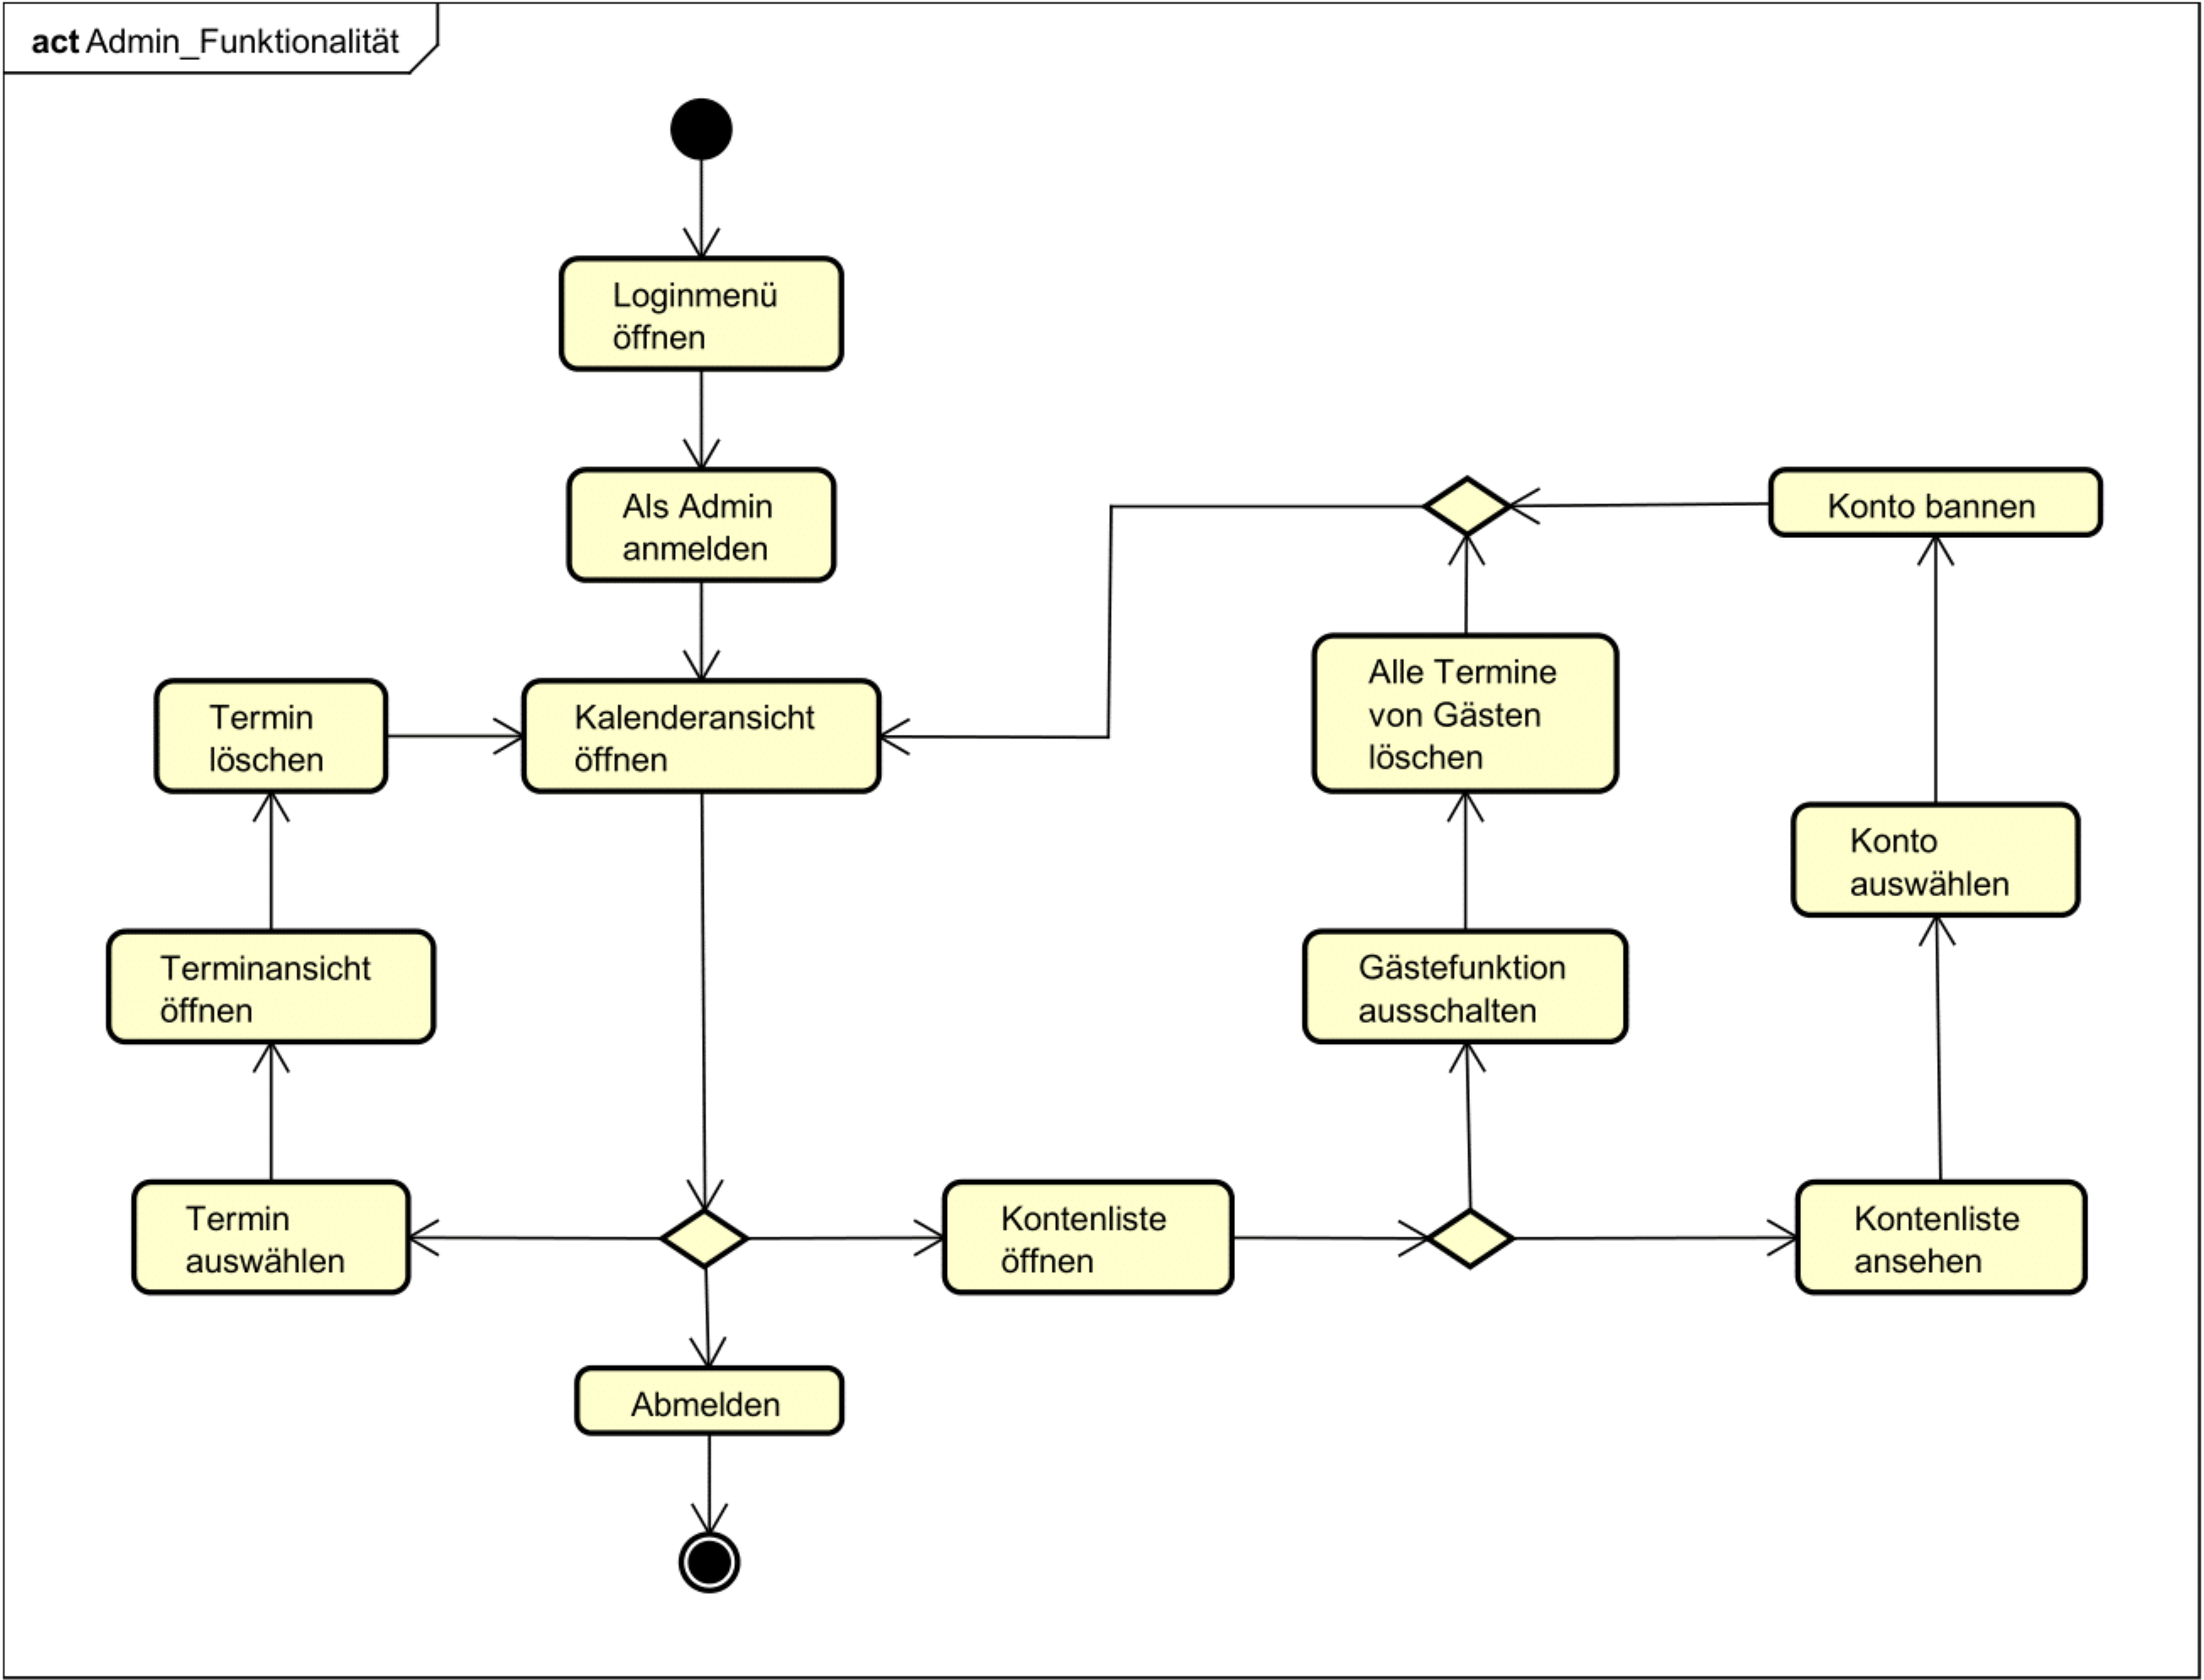
\includegraphics[width=\textwidth]{figures/activitydiagrams/adminfunk}
    \caption{Aktivitätsdiagramm für die Admin-Funktionalität}
    \label{fig:activity_diagram_admin}
\end{figure}
\clearpage
\subsection{Anmeldeprozess}

In Abbildung \ref{fig:activity_diagram_login} ist das Aktivitätsdiagramm für den Anmeldeprozess dargestellt,
welches die Musskriterien \ref{MK2} und \ref{MK17} abdeckt, sowie die Produktfunktionen \ref{F20} und \ref{F100}.
\begin{figure}[ht]
    \centering
    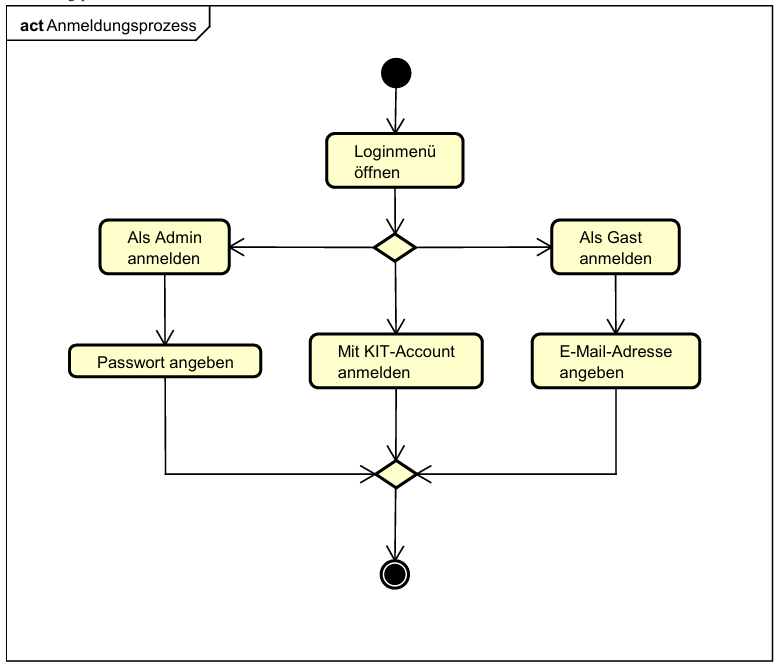
\includegraphics[width=\textwidth]{figures/activitydiagrams/anmeldeprozess}
    \caption{Aktivitätsdiagramm für den Anmeldeprozess}
    \label{fig:activity_diagram_login}
\end{figure}
\clearpage
\subsection{Termin erstellen}

In Abbildung \ref{fig:activity_diagram_booking} ist das Aktivitätsdiagramm für das Erstellen eines Termins dargestellt,
welches die Musskriterien \ref{MK2}, \ref{MK3}, \ref{MK5}, \ref{MK6}, \ref{MK9}, \ref{MK10}, \ref{MK12} und \ref{MK13} abdeckt,
sowie die Produktfunktionen \ref{F20}, \ref{F30} und \ref{F40}.
\begin{figure}[ht]
    \centering
    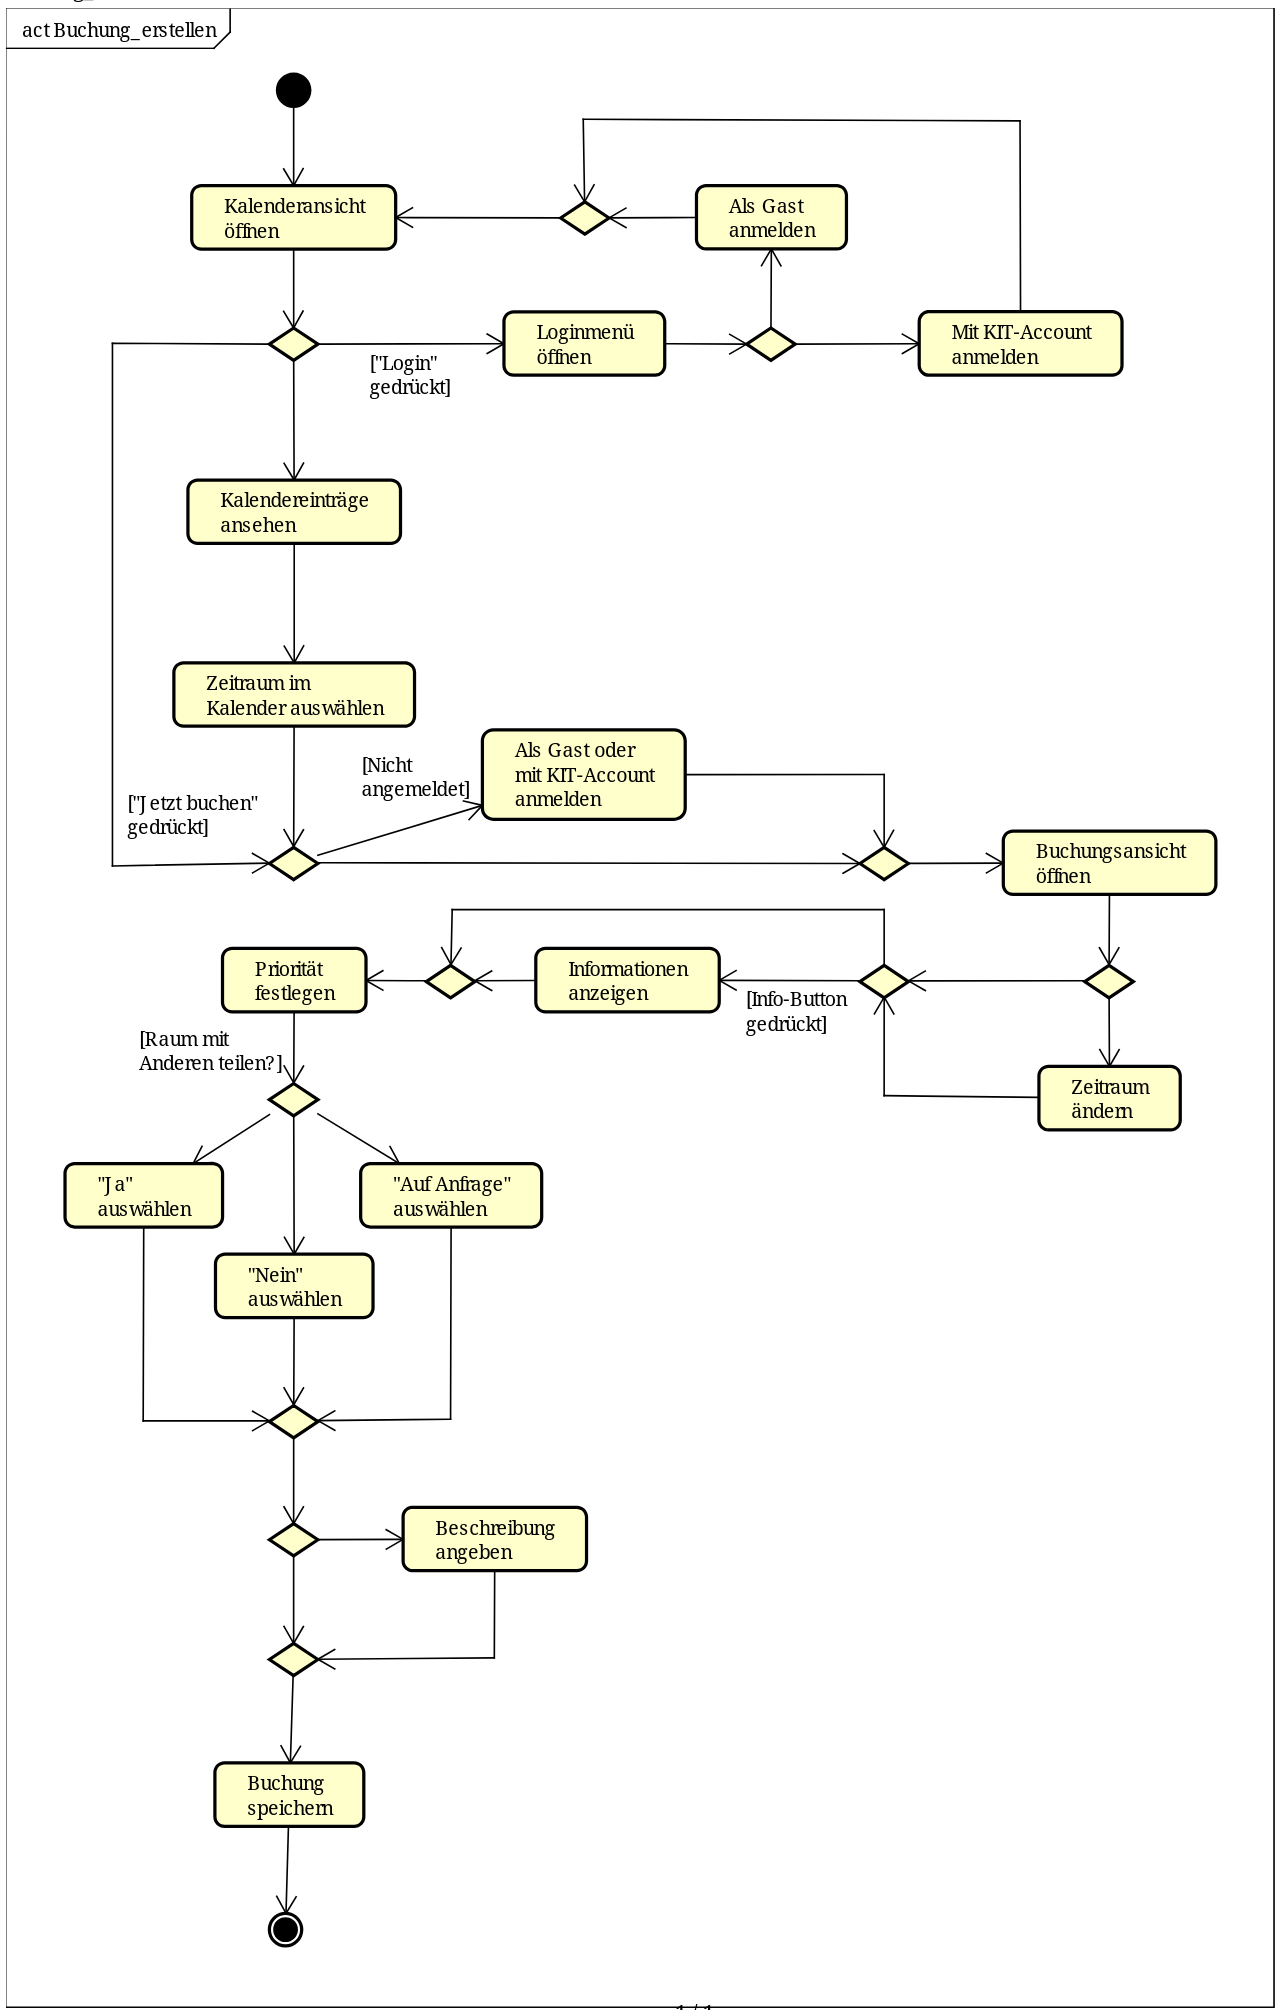
\includegraphics[width=0.6\textwidth]{figures/activitydiagrams/buchungerstellen}
    \caption{Aktivitätsdiagramm für das Erstellen eines Termins}
    \label{fig:activity_diagram_booking}
\end{figure}


\clearpage
\subsection{Termine verwalten}
In Abbildung \ref{fig:activity_diagram_booking_manage} ist das Aktivitätsdiagramm für das Verwalten von Terminen dargestellt,
welches die Musskriterien \ref{MK2}, \ref{MK11} und \ref{MK16} abdeckt, sowie die Produktfunktionen \ref{F20} und \ref{F90}.
\begin{figure}[ht]
    \centering
    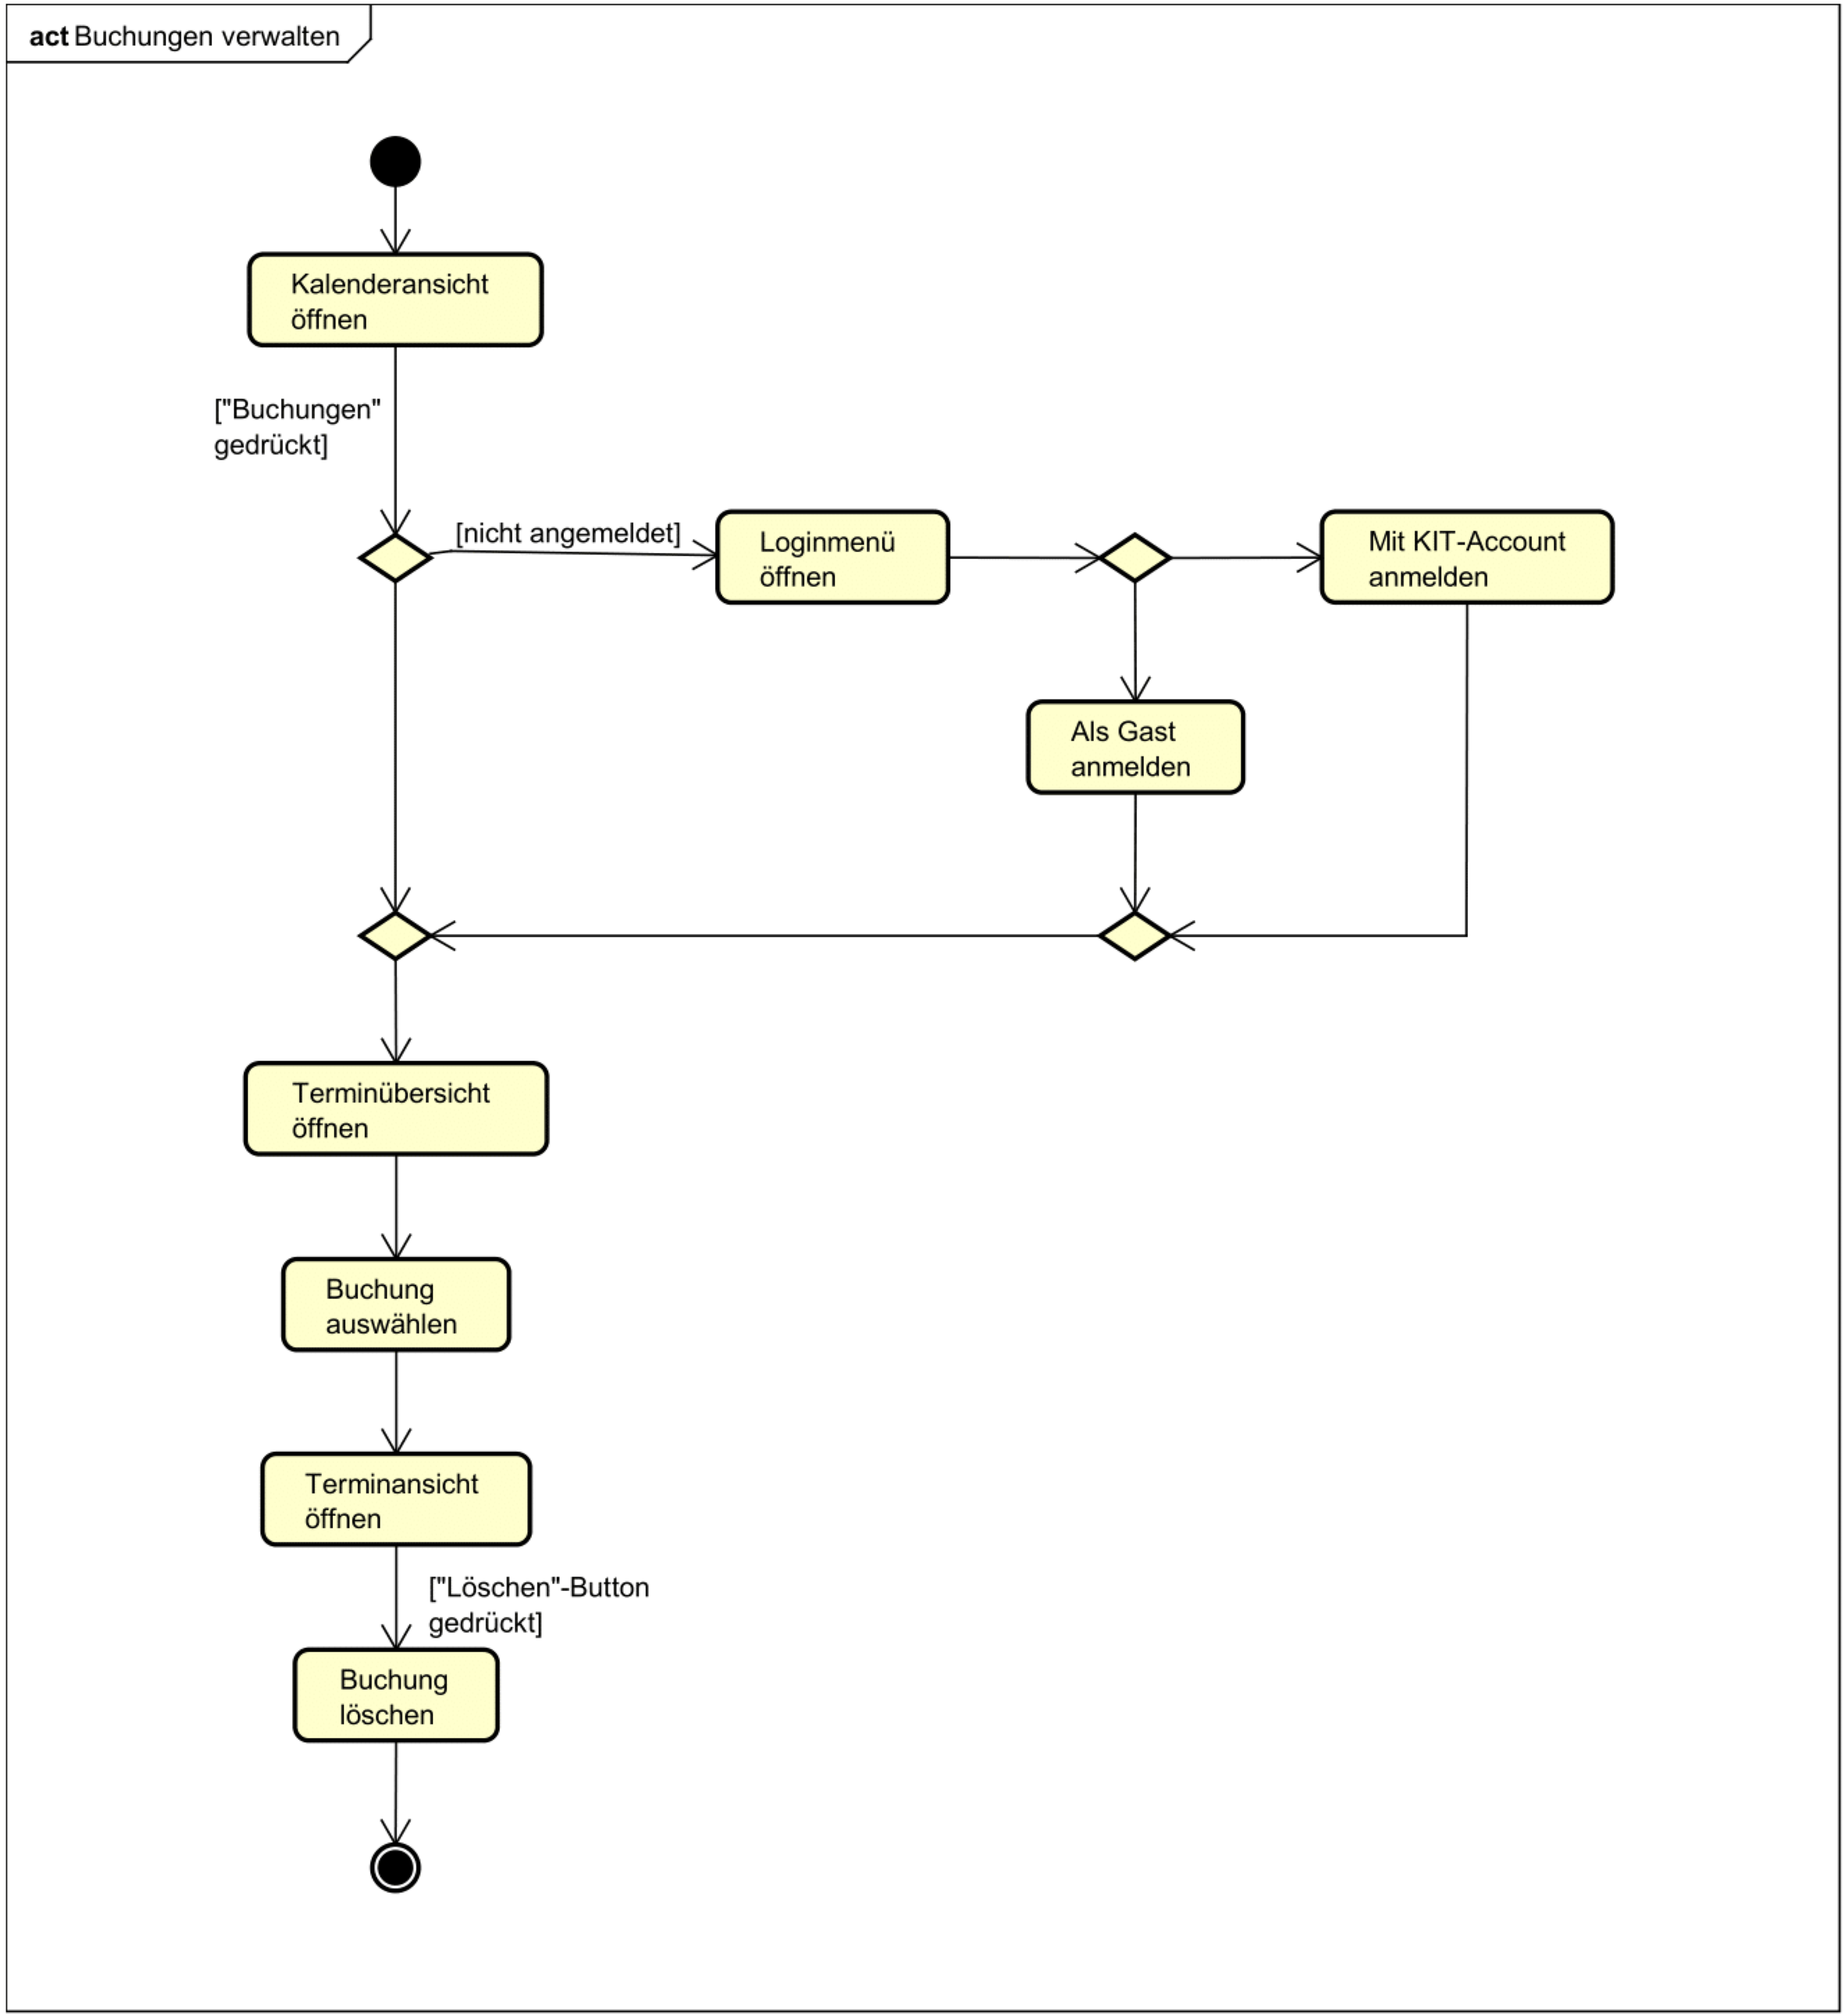
\includegraphics[width=0.8\textwidth]{figures/activitydiagrams/buchungverwalten}
    \caption{Aktivitätsdiagramm für das Verwalten von Terminen}
    \label{fig:activity_diagram_booking_manage}
\end{figure}

\clearpage
\subsection{Termin Ansicht}
In Abbildung \ref{fig:activity_diagram_calendar} ist das Aktivitätsdiagramm für die Ansicht \textit{Termin} dargestellt,
welches die Musskriterien \ref{MK2}, \ref{MK5}, \ref{MK8}, \ref{MK16}, \ref{MK17} und \ref{MK19} abdeckt,
sowie die Produktfunktionen \ref{F20}, \ref{F50}, \ref{F90}, \ref{F100} und \ref{F130}.
\begin{figure}[ht]
    \centering
    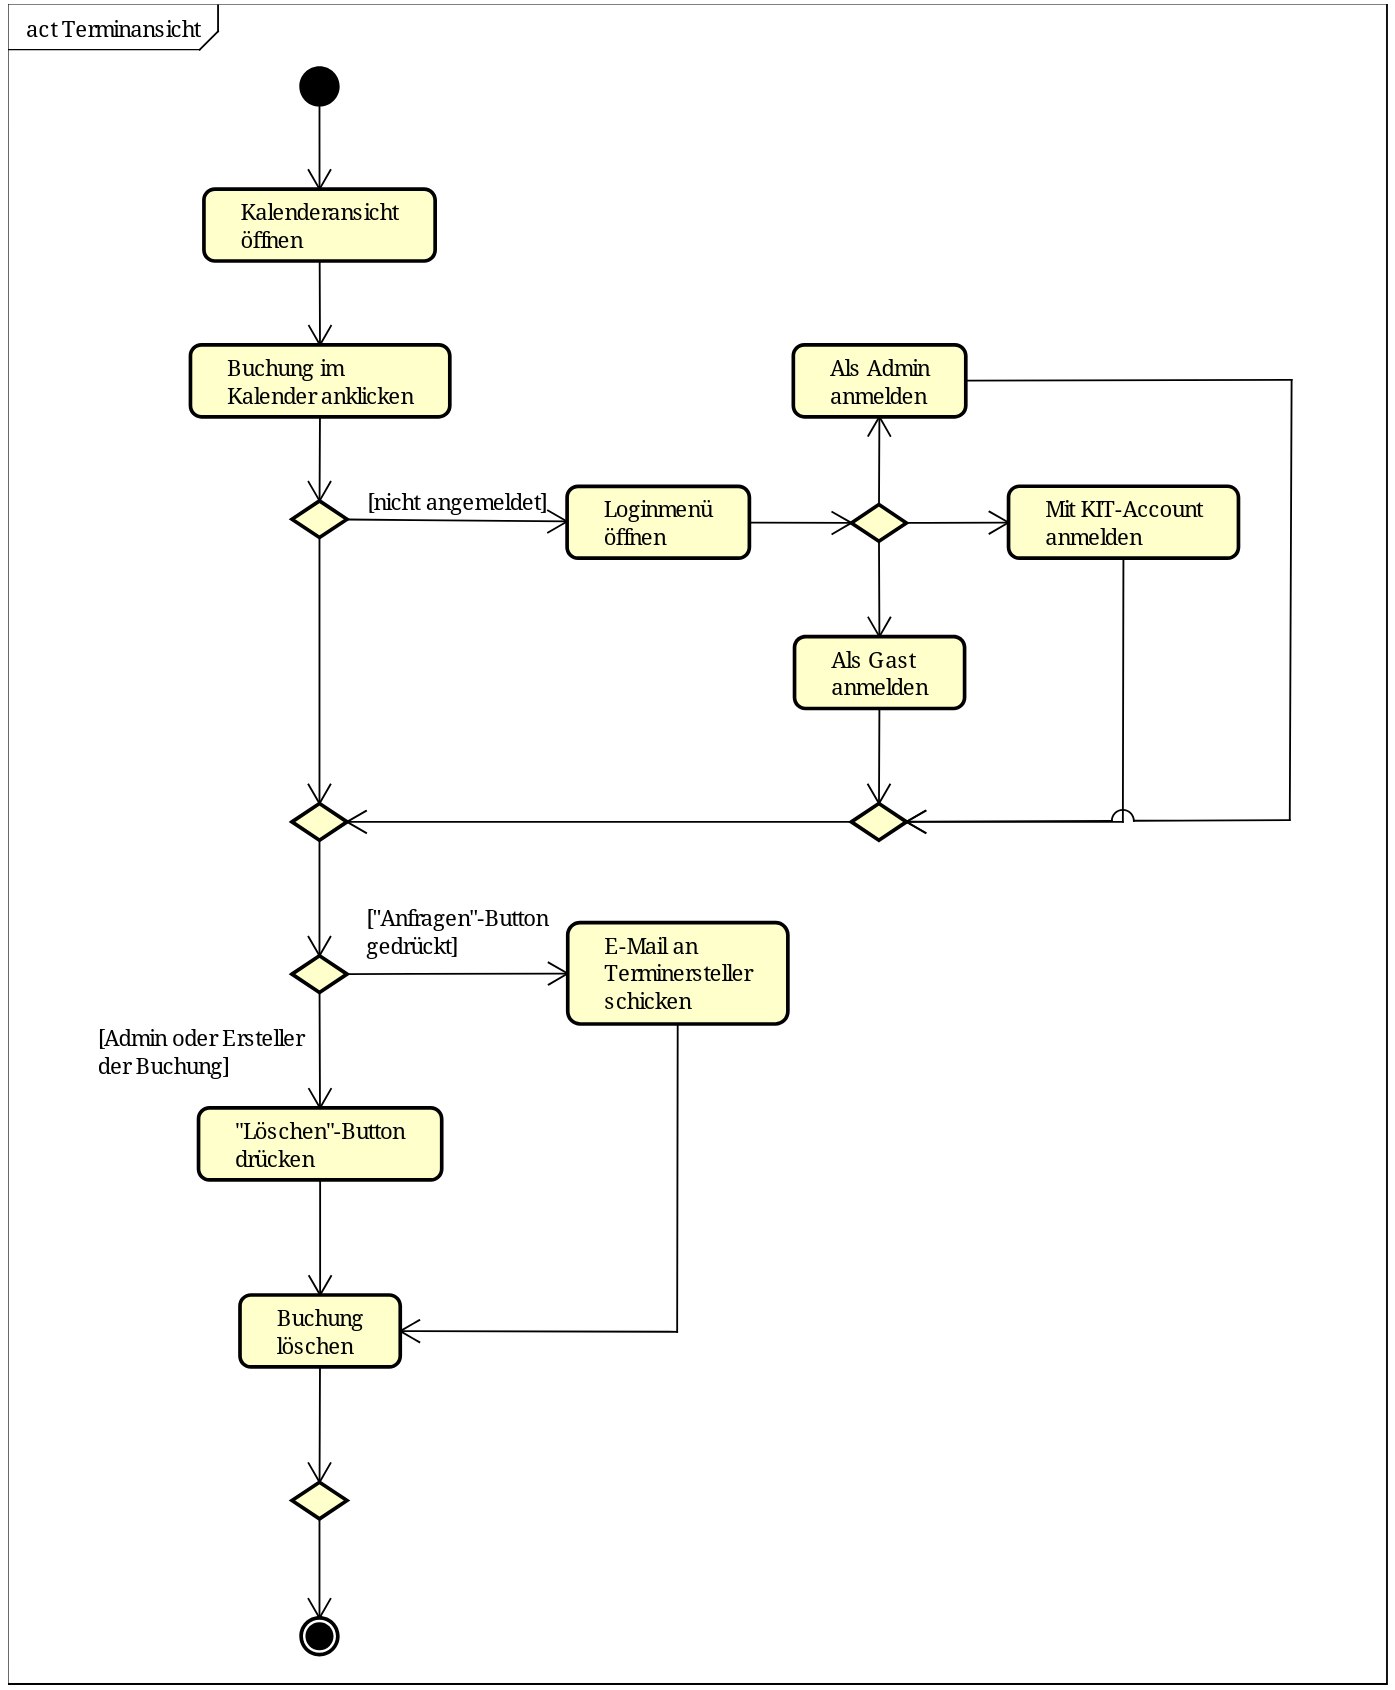
\includegraphics[width=0.8\textwidth]{figures/activitydiagrams/terminansicht}
    \caption{Aktivitätsdiagramm für die Ansicht \textit{Termin}}
    \label{fig:activity_diagram_calendar}
\end{figure}
%!TEX root = ../Pflichtenheft.tex

% Kapitel 4
%-------------------------------------------------------------------------------

\chapter{Produktfunktionen}
\label{chap:product_functions}

\iffalse
In Abhängigkeit von den gewählten Konzepten erfolgt hier eine Konkretisierung
und Detaillierung der Funktionen aus den Use-Case-Diagrammen und ggf. dem
Angebot.

Die Produktfunktionen müssen die Kriterien aus den Zielbestimmungen abdecken.
Dabei kann es je nach Kriterium eine oder mehrere Funktionen geben.
Das nachfolgende Format sollte für einige Funktionsbeschreibungen übernommen werden:

Beispiel:\\
\begin{function}{10}{Lagerverwaltung}
    \item[Anwendungsfall:] Automatisches Einlagern
    \item[Anforderung:] \lfk{20} (Wenn kein Lastenheft vorhanden, dann Kriterium aus den Zielbestimmungen, z.B.: \ref{RM1})
    \item[Ziel:] Ein Reifen erscheint am Systemeingang (Scanner), erhält einen Lagerplatz
    zugewiesen und wird dort eingelagert.
    \item[Vorbedingung:] Das Scannen des Barcode-Reifens muss erfolgreich sein, sonst kann
    der Typ nicht ermittelt werden. Solche unbekannten Reifen werden direkt in den
    Überlauf gefördert.
    \item[Nachbedingung Erfolg:] Reifen ist physikalisch eingelagert und logisch in der
    Datenbank verbucht.
    \item[Nachbedingung Fehlschlag:] Der Reifen wurde infolge gestörter Fördermechanik
    nicht eingelagert (liegt im Überlauf) oder produzierte aufgrund inkonsistenter
    Datenbank einen `Platz belegt` - Fehler beim Anfahren eines irrtümlich
    als frei angenommenen Platzes.
    \item[Akteure:] ~Produktion
    \item[Auslösendes Ereignis:] SPS meldet der Steuerung, dass am Eingangsscanner ein
    Reifen mit Seriennummer X des Typs Y eingetroffen ist.
    \item[Beschreibung:] ~
    \begin{enumerate}
      \item Reifentypinformationen ermitteln (besonders Höhe des Reifens bei Wahl zwischen unterschiedlich hohen Lagerplätzen wichtig).
      \item Alle Module ermitteln, die\\
    - Platz auf den Einlagerstichen haben\\
    - momentan nicht im Störungszustand sind\\
    -  freie Lagerplätze in der geforderten Höhe aufweisen.
      \item Lagerplatz nach Gleichverteilungsgrundsatz bestimmen.
      \item Reifen auf den Einlagerstich des gewählten Moduls befördern.
      \item Sobald er auf dem vordersten Platz des Einlagerstichs steht, dem Modul den Befehl zur Reifenaufnahme und Einlagerung auf den gewählten Platz schicken.
    \end{enumerate}
    \item[Erweiterung:] (optional)\\
        2a Zur Effizienzsteigerung auch Module ansteuern, die momentan keinen Platz auf
        den Einlagerstichen haben, aber wahrscheinlich so schnell einlagern, dass der
        Reifen nach der Fahrtzeit zum Modul auf den Stich eingelagert werden kann
        (Überwachung des `Unterwegsbestandes` an Reifen für ein bestimmtes
        Modul).\\
        3a Lagerplatz des Reifens möglichst nah zum Einlagerstich im RBG wählen	(kürzere RBG-Fahrtzeiten).
    \item[Alternativen:] (optional)\\
        2a Wenn kein Lagerplatz gefunden wird, Reifen zum Überlauf schicken (der
        Einlagerförderer wird niemals angehalten!).
\end{function}
\fi

\begin{function}{10}{Landeseite}
    \item[Anwendungsfall:] Initiales besuchen der Webseite
    \item[Anforderung:]~\ref{RM1}, ~\ref{RW1}, ~\ref{RM4}
    \item[Ziel:] Dem Benutzer wird ohne Anmeldung die Kalenderansicht gezeigt.
    \item[Vorbedingung:] Der Benutzer hat eine Internetverbindung und hat im \gls{Browser}~die Webseite geöffnet.
    \item[Nachbedingung Erfolg:] Der Benutzer sieht die Kalenderansicht mit zukünftigen Reservierungen.
    \item[Nachbedingung Fehlschlag:] Der Benutzer ist nicht in der Lage mit der Webseite weiter zu interagieren.
    \item[Auslösendes Ereignis:] Der Benutzer nutzt seinen \gls{Browser}~, um die Webseite aufzurufen.
    \item[Beschreibung:]~
    \begin{enumerate}
        \item Der Benutzer navigiert in seinem Browser auf die Webseite.
        \item Die Landeseite lädt und zeigt dem Benutzer die Kalenderansicht an.
        \item Ebenfalls wird dem Benutzer wird eine Schaltfläche angezeigt zum Erstellen eines Termines, sowie zum Anmelden/Registrieren.
    \end{enumerate}
    \item[Erweiterung:] Sollte es mehr als ein Arbeitsraum geben, so sollte hier vom Nutzer die Auswahl getroffen werden, bevor die Kalenderansicht angezeigt wird.
\end{function}

% require at least 10 lines, otherwise pagebreak
\needspace{10\baselineskip}

\begin{function}{20}{Anmelden}
    \item[Anwendungsfall:] Anmelden bzw.\ Registrieren
    \item[Anforderung:]~\ref{RM2}
    \item[Ziel:] Der Benutzer kann sich mit seinem KIT-Konto oder einem lokalen Gastkonto anmelden.
    \item[Vorbedingung:] Der Benutzer hat eine Internetverbindung und die Anwendung ist gestartet.
    \item[Nachbedingung Erfolg:] Der Benutzer ist angemeldet und kann Ereignisse ansehen und bearbeiten.
    \item[Nachbedingung Fehlschlag:] Der Benutzer ist nicht angemeldet und kann keine Ereignisse ansehen oder bearbeiten.
    \item[Auslösendes Ereignis:] Der Benutzer öffnet die Anwendung und versucht, mit einem Ereignis zu interagieren.
    \item[Beschreibung:] ~
    \begin{enumerate}
        \item Der Benutzer wählt in einem Dialog die Anmeldemethode aus.
        \item Sollte dieser noch keinen Account haben, so wird statt eine Anmeldung eine Registrierung vollzogen.
        \item Der Benutzer wird, falls nötig, auf die KIT-Login-Seite weitergeleitet.
        \item Falls keine lokale Anmeldung gewählt wurde, gibt der Benutzer seine Zugangsdaten ein.
        \item Die Anwendung überprüft die Zugangsdaten und meldet den Benutzer an.
        \item Der Benutzer wird zur nächsten Seite weitergeleitet.
    \end{enumerate}
\end{function}
\begin{function}{20}{Reservierung}

\begin{function}{30}{Reservierung}
    \item[Anwendungsfall:] Reservierung
    \item[Anforderung:]~\ref{RM3},~\ref{RM8},~\ref{RM9} und~\ref{RM10}
    \item[Ziel:] Der Benutzer kann einen Raum reservieren.
    \item[Vorbedingung:] Der Benutzer ist angemeldet und hat eine Internetverbindung.
    \item[Nachbedingung Erfolg:] Eine Reservierung wird gespeichert und der Benutzer zur Buchungsseite weitergeleitet.
    \item[Nachbedingung Fehlschlag:] Die Reservierung wird nicht gespeichert und der Benutzer erhält eine Fehlermeldung.
    \item[Auslösendes Ereignis:] Der Benutzer wählt einen Raum und einen Startzeitpunkt.
    \item[Beschreibung:] ~
    \begin{enumerate}
        \item Der Benutzer prüft einen Start- und Endzeitpunkt und kann sie gegebenenfalls anpassen.
        \item Der Benutzer gibt optional eine Beschreibung an.
        \item Der Benutzer gibt an, ob er bereit ist, die Reservierung zu teilen.
        \item Der Benutzer gibt optional eine E-Mail-Adresse an, um über Änderungen informiert zu werden.
        \item Falls eine E-Mail-Adresse angegeben wurde, kann der Benutzer diese als in der Oberfläche sichtbar oder unsichtbar markieren.
        \item Der Benutzer bestätigt seine Eingaben.
        \item Die Anwendung prüft, ob der Raum in dem Zeitraum verfügbar ist.
        \item Falls ja, wird die Reservierung gespeichert und der Nutzer weitergeleitet.
              Wenn nötig, wird eine E-Mail an die Ersteller überschriebener Reservierungen gesendet.
    \end{enumerate}
\end{function}

\begin{function}{40}{Löschen von Terminen}
    \item[Anwendungsfall:] Löschen von Terminen
    \item[Anforderung:] ~\ref{RM16}
    \item[Ziel:] Der Administrator kann bestehende Termine löschen.
    \item[Vorbedingung:] Der Administrator ist angemeldet.
    \item[Nachbedingung Erfolg:] Der Termin wird aus dem System entfernt und der Administrator erhält eine Bestätigungsmeldung.
    \item[Nachbedingung Fehlschlag:] Der Termin wird nicht gelöscht und der Administrator erhält eine Fehlermeldung.
    \item[Auslösendes Ereignis:] Der Administrator wählt einen Termin aus, den er löschen möchte.
    \item[Beschreibung:] ~
    \begin{enumerate}
        \item Der Administrator öffnet die Liste der bestehenden Termine.
        \item Der Administrator wählt den Termin aus, den er löschen möchte.
        \item Der Administrator wird gefragt, ob er den Termin wirklich löschen möchte (Bestätigungsabfrage).
        \item Falls der Administrator bestätigt, wird der Termin gelöscht.
        \item Eine Bestätigungsmeldung wird angezeigt (z. B. "Termin erfolgreich gelöscht").
    \end{enumerate}
\end{function}

\begin{function}{50}{Deaktivierung von Gastbenutzern}
    \item[Anwendungsfall:] Deaktivierung von Gastbenutzern
    \item[Anforderung:] ~\ref{RM16}
    \item[Ziel:] Der Administrator kann Gastbenutzer deaktivieren.
    \item[Vorbedingung:] Der Administrator ist angemeldet und hat die entsprechenden Berechtigungen.
    \item[Nachbedingung Erfolg:] Der Gastbenutzer wird deaktiviert und ist nicht mehr im System aktiv.
    \item[Nachbedingung Fehlschlag:] Der Gastbenutzer bleibt aktiv und der Administrator erhält eine Fehlermeldung.
    \item[Auslösendes Ereignis:] Der Administrator wählt einen Gastbenutzer aus, den er deaktivieren möchte.
    \item[Beschreibung:] ~
    \begin{enumerate}
        \item Der Administrator öffnet die Liste der Gastbenutzer.
        \item Der Administrator wählt einen Gastbenutzer aus, den er deaktivieren möchte.
        \item Der Administrator bestätigt die Deaktivierung.
        \item Der Gastbenutzer wird deaktiviert und aus der aktiven Liste entfernt.
        \item Eine Bestätigungsmeldung wird angezeigt (z. B. "Gastbenutzer erfolgreich deaktiviert").
    \end{enumerate}
\end{function}

\begin{function}{60}{Benachrichtigung bei freiem Raum}
    \item[Anwendungsfall:] Benachrichtigung über freigewordenen Raum
    \item[Anforderung:] ~\ref{RM17}
    \item[Ziel:] Die Anwendung informiert Benutzer, wenn ein Raum wieder frei wird.
    \item[Vorbedingung:] Der Benutzer hat sich für den Raum interessiert und hat eine Benachrichtigung angefordert.
    \item[Nachbedingung Erfolg:] Der Benutzer wird über die Freigabe des Raums per E-Mail oder Benachrichtigung informiert.
    \item[Nachbedingung Fehlschlag:] Der Benutzer erhält keine Benachrichtigung, und eine Fehlermeldung wird angezeigt.
    \item[Auslösendes Ereignis:] Der Raum wird freigegeben, nachdem eine vorherige Reservierung aufgehoben oder geändert wurde.
    \item[Beschreibung:] ~
    \begin{enumerate}
        \item Der Benutzer wählt aus ob er für den Raum Benachrichtigungen erhalten möchte, wenn er wieder frei wird.
        \item Der Benutzer gibt eine E-Mail-Adresse an, um die Benachrichtigungen zu empfangen (Sollte keine hinterlegt sein über KIT-Account).
        \item Sobald der Raum wieder verfügbar ist, prüft das System, ob Benutzer für den Raum eine Benachrichtigung angefordert haben.
        \item Den betroffenen Benutzern wird eine E-Mail oder Benachrichtigung zugeschickt, dass der Raum nun wieder verfügbar ist.
        \item Eine Bestätigung der erfolgreichen Benachrichtigung wird im System protokolliert.
    \end{enumerate}
\end{function}

\begin{function}{70}{Anzeige des Raumstatus}
    \item[Anwendungsfall:] Anzeige des Raumstatus
    \item[Anforderung:] ~\ref{RM18}
    \item[Ziel:] Die Anwendung stellt den Raumstatus, einschließlich der aktuellen Belegung und Priorität, übersichtlich dar.
    \item[Vorbedingung:] Der Benutzer ist nicht eingeloggt.
    \item[Nachbedingung Erfolg:] Der Raumstatus wird auf einer öffentlichen Seite korrekt angezeigt, inklusive Belegung und Priorität (z. B. durch farbige Banner).
    \item[Nachbedingung Fehlschlag:] Der Raumstatus wird nicht angezeigt oder ist unvollständig.
    \item[Auslösendes Ereignis:] Der Benutzer öffnet die Seite mit den Informationen zu den Räumen.
    \item[Beschreibung:] ~
    \begin{enumerate}
        \item Der Benutzer öffnet die Seite.
        \item Der Raum wird mit dem entsprechenden Status angezeigt, der die aktuelle Belegung widerspiegelt.
        \item Falls der Raum belegt ist, wird dies deutlich sichtbar gemacht (z. B. durch einen roten Banner oder ein entsprechendes Symbol).
        \item Falls der Raum eine höhere Priorität hat, wird diese Information ebenfalls angezeigt, z. B. durch einen farbigen Banner oder ein Symbol, das den Raum hervorhebt.
        \item Der Raumstatus ist für alle Benutzer sichtbar, ohne dass eine Anmeldung erforderlich ist.
    \end{enumerate}
\end{function}

\begin{function}{80}{Stornierung einer Reservierung}
    \item[Anwendungsfall:] Stornierung einer Reservierung
    \item[Anforderung:] ~\ref{RM14}
    \item[Ziel:] Der Benutzer kann eine bestehende Reservierung stornieren.
    \item[Vorbedingung:] Der Benutzer ist angemeldet und hat eine aktive Reservierung.
    \item[Nachbedingung Erfolg:] Die Reservierung wird storniert und der Benutzer erhält eine Bestätigungsmeldung.
    \item[Nachbedingung Fehlschlag:] Die Reservierung wird nicht storniert und der Benutzer erhält eine Fehlermeldung.
    \item[Auslösendes Ereignis:] Der Benutzer wählt die Option zur Stornierung einer bestehenden Reservierung.
    \item[Beschreibung:] ~
    \begin{enumerate}
        \item Der Benutzer öffnet die Seite mit seinen aktuellen Reservierungen.
        \item Der Benutzer wählt die Reservierung aus, die er stornieren möchte.
        \item Der Benutzer bestätigt die Stornierung der Reservierung (z. B. durch Klick auf „Reservierung stornieren“).
        \item Eine Bestätigungsabfrage erscheint, in der der Benutzer die Stornierung bestätigen muss.
        \item Falls der Benutzer bestätigt, wird die Reservierung storniert.
        \item Das System aktualisiert die Raumverfügbarkeit und zeigt dem Benutzer eine Bestätigungsmeldung (z. B. "Reservierung erfolgreich storniert").
        \item Der Benutzer erhält ggf. eine E-Mail oder eine Benachrichtigung über die Stornierung (optional).
    \end{enumerate}
\end{function}


%!TEX root = ../Pflichtenheft.tex

\chapter{Produktdaten}
\label{chap:product_data}

\iffalse
Die langfristig zu speichernden Daten sind aus Benutzersicht detaillierter zu beschreiben.
Dabei bietet sich eine formale Beschreibung an, um eine größere Präzisierung zu erreichen.
Es sollte eine Menge an erwarteten Daten angegeben werden.

Es kann die Darstellung gemäß Beispiel verwendet werden (alternativ kann auch ein Klassendiagramm mit entsprechender Beschreibung erstellt werden):\\

\begin{data}{10}{Lagerdaten}
	Daten der Lagerplätze (max. 5.000):\\
	-  Modulnummer,\\
	-  Regalseite,\\
	-  Regalspalte,\\
	-  Regalzeile,\\
	-  Fachhöhe,\\
	-  Platzsperre (0 = nicht gesperrt, 1 = gesperrt für Einlagerung, 2 = gesperrt
	   für Auslagerung, 3 = gesperrt für alle Zugriffe),\\
	-  Reifenstatus (0 = frei,1 = reserviert für Einlagerung, 2= belegt, 3 =
	   reserviert für Auslagerung),\\
	-  Reifenseriennummer.\\
\end{data}

\begin{data}{20}{Moduldaten}
	Daten der Module (max. 20):\\
	-  Modulnummer,\\
	-  Sperrkennzeichen (0 = nicht gesperrt, 1 = gesperrt für Einlagerung, 2 =
	   gesperrt für Auslagerung, 3 = gesperrt für alle Zugriffe),\\
	-  maximale Kapazität,\\
	-  freie Kapazität,\\
	-  belegte Plätze (ergibt sich aus Status und Zahl der zugeordneten
	   Lagerplätze, wird aus Geschwindigkeitsgründen allerdings redundant
	   mitgeführt).
\end{data}
\fi

Die Anwendung verwendet den Server als zentralen Speicherort für alle Daten.
Die Daten werden in einer \gls{PostgreSQL}-Datenbank gespeichert.
Auf dem Client werden nur temporäre Daten gespeichert, die für die Funktionalität der Anwendung notwendig sind.

\improvement{Das LaTeX-Template bietet für diese Sektion ein anderes Format an. Ich hab es nicht schön gekriegt, deshalb habe ich es so gelöst.}

\subsection*{Clientdaten}
\begin{itemize}
    \item Anmeldungscookie (falls der Benutzer anonym angemeldet ist)
    \item Zustand der Anwendung (z.B.\ aktuelle Seite, geöffnete Dialoge)
\end{itemize}

\subsection*{Serverdaten}
\begin{itemize}
    \item Benutzerdaten
    \begin{itemize}
        \item Benutzername (oder \textit{Anonym} für anonyme Benutzer)
        \item (optional) E-Mail-Adresse
        \item OAuth- oder Cookie-Token
    \end{itemize}
    \item Ereignisdaten
    \begin{itemize}
        \item Start- und Endzeitpunkt \unsure{Wie kodieren wir die Zeit? Fixe Slots oder Unix-Timestamp?}
        \item Beschreibung
        \item Raum
        \item Ersteller
        \item Priorität
        \item Kollaborativität
        \item (optional) E-Mail-Adresse
        \item Sichtbarkeit der E-Mail-Adresse
    \end{itemize}
    \item Raumdaten
    \begin{itemize}
        \item Raumname
        \item Raumbeschreibung
        \item Raumbild
    \end{itemize}
\end{itemize}
%!TEX root = ../Pflichtenheft.tex

% Kapitel 6
%-------------------------------------------------------------------------------

\chapter{Nichtfunktionale Anforderungen}
\label{chap:non_functional_req}

\iffalse
In diesem Kapitel wird festgelegt, welche Qualitätsmerkmale das zu entwickelnde
Produkt in welcher Qualitätsstufe besitzen soll. Anschließend werden die als am
wichtigsten bezeichneten Qualitätsmerkmale operationalisiert, d.h. in konkrete
Produktanforderungen detailliert, falls sie nicht als allgemeine Richtlinie (z.
B. Standard, Norm) zur Verfügung gestellt werden können.


Die oben als am wichtigsten bezeichneten Qualitätsmerkmale werden im Folgenden
operationalisiert, d.h. in konkrete Produktanforderungen detailliert oder es
wird angegeben, welche Richtlinie (z. B. Standard, Norm) einzuhalten ist. Diese
Qualitätsanforderungen werden wie im Beispiel definiert. Zu prüfen ist, ob die
gewünschte Qualität mit den in Produktdaten genannten Datenmengen erreicht
werden kann.
\fi


\notfunctional{1}{Die Anwendung soll schnell und einfach bedienbar sein.}
\notfunctional{2}{Die Anwendung soll auf mobilen sowie Desktop-Endgeräten ohne Einschränkungen nutzbar sein.}
\notfunctional{3}{Die Anwendung soll in allen gängigen Browsern lauffähig sein. Insbesondere beinhaltet dies Firefox und Chrome auf Desktop- und Android-Geräten und Safari auf iOS.}
\notfunctional{4}{Die Anonymität der Nutzer soll so weit wie möglich gewährleistet werden.}
\notfunctional{5}{Für Nutzer mit Sehschwäche soll die Anwendung durch Kompatibilität mit Screenreadern und kontrastreiche Farbgebung gut bedienbar sein.}
\notfunctional{6}{Die Anwendung soll in verschiedenen Sprachen dargestellt werden können, insbesondere Deutsch und Englisch.}
\notfunctional{7}{Die Anwendung soll auf mobilen sowie Desktop-Endgeräten ohne Einschränkungen nutzbar sein.}
\notfunctional{8}{x}

%!TEX root = ../Pflichtenheft.tex

\chapter{Benutzeroberfläche}
\label{chap:ui}

In diesem Kapitel kann, an euer Projekt angepasst, die Benutzeroberfläche durch UI Mocks beschrieben werden.



%!TEX root = ../Pflichtenheft.tex

% Kapitel 10
% Die Unterkapitel können auch in separaten Dateien stehen,
% die dann mit dem \include-Befehl eingebunden werden.
%-------------------------------------------------------------------------------

\chapter{Technische Produktumgebung}
\label{chap:tech_env}

\section{Entwicklungsumgebung}

\begin{itemize}
    \item Devcontainer für reproduzierbare Entwicklungsumgebung
    \item IntelliJ IDEA als IDE und LaTex-Editor
    \item pdfLaTeX zur Kompilierung des Dokuments
    \item Git zur Versionskontrolle
    \item GitHub Actions für CI/CD (inkl. Tests und Dokumentation)
    \item GitHub Packages zur Speicherung generierter Docker-Images
\end{itemize}

\section{Hardware}

\subsection{Backend}

\begin{itemize}
    \item AMD64-kompatibler Prozessor (emuliert in einer VM)
    \item mindestens 1 GB RAM
\end{itemize}

\subsection{Frontend}

\begin{itemize}
    \item Beliebiges (mobiles) Gerät mit Internetzugang
\end{itemize}

\section{Software}

\subsection{Backend}

\begin{itemize}
    \item Ubuntu Linux 24.04 LTS als Betriebssystem
    \item Docker zur Containerisierung der Anwendung
    \item PostgreSQL als Datenbank (in einem eigenen Container)
    \item Applikations-Container (gebaut in CI)
    \item Spring Boot mit Java 21 als Backend-Framework
    \todo[inline]{Wie machen wir HTTPS? Mit Spring oder per NGINX/Caddy? Wie kriegen wir Domäne, Zertifikat, ...?}
\end{itemize}

\subsection{Frontend}

\begin{itemize}
    \item Pure HTML mit JavaScript zur Interaktivität um maximale Kompatibilität zu gewährleisten
    \item DaisyUI als CSS-Framework
    \item FullCalendar für die Kalenderansicht
    \item Moderner Browser (Chrome, Firefox, Safari, Edge) zur vollen Funktionalität
\end{itemize}

\section{Schnittstellen}

\begin{itemize}
    \item SSR (Server-Side Rendering) generiert HTML-Dateien
    \item HTML-Forms zur Interaktion mit dem Backend
    \item Minimale REST-API zum Prüfen auf Verfügbarkeit
    \todo[inline]{Machen wir das?}
\end{itemize}
\chapter{Testfälle und Testeszzenarien}
\label{chap:test}
In diesem Kapitel definieren wir die Testfälle und Testfallszenarien.

\section{Basis-Testfälle}

Jeder Produktfunktion entspricht einem Basis-Testfall. Die Basis-Testfälle sind uten aufgelistet.


\begin{table}[htbp]

  \centering
%    \caption{Überblick von allen Funktionen.}
  \begin{tabularx}{\textwidth}{ l|X|l }
      \textbf{Nr.} & \textbf{Beschreibung} & \textbf{Funktion} \\ \hline\hline
      ⟨T10⟩ & Landeseite besuchen &\ref{F10}\\
      ⟨T20⟩ & Login &\ref{F20} \\
      ⟨T30⟩ & Abmelden &\ref{F30} \\
      ⟨T40⟩ & Reservieren &\ref{F40} \\
      ⟨T50⟩ & Löschen von Terminen durch Administratoren &\ref{F50} \\
      ⟨T60⟩ & Deaktivieren eines Kontos &\ref{F60} \\
      ⟨T70⟩ & Benachrichtigung bei freiem Raum &\ref{F70} \\
      %⟨T80⟩ & Anzeige des Raumstatus &\ref{F80} \\'
      ⟨T90⟩ & Stornierung einer Reservierung &\ref{F90} \\
      ⟨T100⟩& Login mit Adminkonto &\ref{F100} \\
      ⟨T110⟩ & Deaktivierung von Gastkonten &\ref{F110} \\
      ⟨T120⟩& Öffnungszeiten einstellen &\ref{F120} \\
      ⟨T130⟩& Terminkonfliktauflösung &\ref{F130} \\
  \end{tabularx}\label{tab:test_table}
\end{table}

\pagebreak

\section{Testfallszenarien}
Die Testfallszenarien ergeben sich als Komposition der Basis-Testfälle.\\ \\
\begin{scenario}{10}{Besuch der Landeseite und Anmeldung/Abmeldung}
  \item[Ziel:] Sicherstellen, dass Nutzende die Landeseite aufrufen und sich erfolgreich anmelden bzw.\ abmelden können.
  \begin{enumerate}
    \item Der Nutzende besucht die Landeseite ⟨T10⟩.
    \item Der Nutzende loggt sich ein ⟨T20⟩.
    \item Der Nutzende meldet sich ab ⟨T30⟩.
  \end{enumerate}
\end{scenario}

\begin{scenario}{20}{Reservierung eines Raums und Stornierung}
  \item[Ziel:] Überprüfen, ob Nutzende erfolgreich Termine reservieren können.
  \begin{enumerate}
    \item Der Nutzende besucht die Landeseite ⟨T10⟩.
    \item Der Nutzende meldet sich an ⟨T20⟩.
    \item Der Nutzende wählt einen verfügbaren Raum aus und reserviert diesen ⟨T40⟩.
    \item Buchen ausserhalb der Öffnungszeiten sollte hierbei fehlschlagen.
    \item Der Nutzende storniert die Reservierung ⟨T90⟩.
    \item Andere Nutzende, welchen sich diesen Termin vorgemerkt hatten, werden benachrichtigt, dass der Raum nun Frei ist ⟨T70⟩.
  \end{enumerate}
\end{scenario}

\begin{scenario}{30}{Verwaltung durch das Adminkonto}
  \item[Ziel:] Testen der administrativen Funktionalitäten zum Löschen von Terminen, Deaktivieren von Gastkonten und einstellen der Öffnungszeiten.
  \begin{enumerate}
    \item Ein Admin besucht die Landeseite ⟨T10⟩.
    \item Der Admin meldet sich an ⟨T100⟩.
    \item Der Admin löscht bestehende Termine ⟨T50⟩.
    \item Der Admin deaktiviert die Anmeldung von Gastkonten ⟨T110⟩.
    \item Der Admin ändert die Öffnungszeiten für einen bestimmten Wochentag ⟨T120⟩.
    \item Der Admin öffnet die Ansicht \textit{Kontoliste} und deaktiviert ein Konto ⟨T60⟩.
    \item Der Admin meldet sich ab ⟨T30⟩.
    \item Das Anmelden mit einem Gastkonto sollte jetzt fehlschlagen ⟨T20⟩.
  \end{enumerate}
\end{scenario}

\todo{this is just wrong!}
\begin{scenario}{40}{Termin anzeigen}
  \item[Ziel:] Überprüfen, ob ein Termin richtig.
  \begin{enumerate}
    \item Der Nutzende besucht die Landeseite ⟨T10⟩.
    \item Der Nutzende meldet sich an ⟨T20⟩.
    \item Der Nutzende wählt einen Raum aus und überprüft dessen Status ⟨T20⟩.
  \end{enumerate}
\end{scenario}

\begin{scenario}{50}{Terminkonflikt auflösung}
  \item[Ziel:] Überprüfen, ob ein Terminkonflikt richtig aufgelöst wird.
  \begin{enumerate}
    \item Konto 1 meldet sich an ⟨T20⟩.
    \item Konto 1 erstellt einen Termin, und gibt die zu testende Priorität, Raumteilungsoption und Zeitperiode ein ⟨T20⟩.
    \item Konto 1 meldet sich ab und Konto 2 meldet sich an.
    \item Konto 2 erstellt einen Termin, welcher den anderen überlappt.
    \item Es wird überprüft, ob die erwartete Konfliktauflösung stattgefunden hat und ggf.\ die dafür benötigten E-Mails versendet wurden ⟨T130⟩.
  \end{enumerate}
\end{scenario}








\printglossaries

%------Ende des Dokumentes------------------------------------------------------
\end{document}
